\documentclass[9pt]{beamer}
% \documentclass[notes, handout, 9pt]{beamer}
% \documentclass[handout, 9pt]{beamer}

\usepackage{import}
\subimport{../}{preamble.tex}
\subimport{../}{beamer-theme.tex}
\usepackage{svg}

% Location for all figures / pictures
\graphicspath{{pictures/}{figures/}}

% % Figures inline
\usepackage{tikz}
\usepackage{pgfplots}
\usetikzlibrary{calc}
\usetikzlibrary{shapes.multipart}
\usetikzlibrary{decorations.pathreplacing}
\usetikzlibrary{arrows.meta}
\usepgfplotslibrary{fillbetween}

%--------------------------------------------------
% Presentation Information
%--------------------------------------------------
\title[Continuous Optimization]{Lagrangian Duality}
\author[]{\textbf{Bart Van Parys}}
\date[]{Fall 2026}
%--------------------------------------------------

\begin{document}

\begin{frame}  

  \maketitle

  \vspace{-2em}
  
    \begin{center}
    \begin{tabular}{lll}
      Instructor : & \textbf{Bart Van Parys} & \textbf{(\href{mailto:mastermath@vanparys.xyz}{mastermath@vanparys.xyz})} \\
    \end{tabular}
  \end{center}
  
\end{frame}

\section{Generalized Duality}

\begin{frame}{Example}

  Consider the linear optimization problem
  \[
    \begin{array}{rl}
      \minimize & f(x) \defn x_1 + x_2 + \dots + x_{3000}\\[0.5em]
      \st & x_1 + 2 x_2 + \dots + 3000 x_{3000}\geq 1 \\[0.5em]
                & 3000 x_1 + 2999 x_2 + \dots + x_{3000} \geq 100
    \end{array}
  \]

  The optimizer is $x^\star$ with optimal value $101/3001$. How to check this ?
  \uncover<2->{
    \vfill
    Combine first and second inequality. For all \emph{feasible} $x$ we must have
    \begin{align*}
      (1+3000)x_1 + (2+2999) x_2 + \dots + (3000+1) x_{3000} & \geq 100+1\\
      3001 ( x_1 + x_2 + \dots + x_{3000} ) & \geq 101 \\
      f(x) & \geq {101}/{3001}
    \end{align*}
  }


  \vfill

  \uncover<3->{
  \begin{tcolorbox}
    \emph{Duality} is \textbf{nothing else} than a generalization of this trick.
  \end{tcolorbox}
  }

\end{frame}

\begin{frame}{General Optimization Problem}

  Let 
  \begin{itemize}
  \item $X \subseteq\Re^n$ be a set of feasible decisions $x$
  \item $f:~\Re^n\to\Re$ be the cost function
  \item $g:~\Re^n\to\Re^m$ be the constraint function
  \item $b\in \Re^m$ be the budget
  \end{itemize}
  
  \vfill

  \begin{tcolorbox}
    \[
      \begin{array}{rl}
        p^\star \defn \inf_x &  f(x) \\[0.5em]
        \st  & x \in X \\[0.5em]
                           & g(x) \succeq_{\Re^m_+} b
      \end{array}
    \]
  \end{tcolorbox}
\end{frame}

\begin{frame}{Playing with Constraints}

  Let $\mc F$ be a set of \emph{non-decreasing (price) functions} $F:\Re^m\to\Re$. That is, 
  \[
    u \succeq_{\Re^m_+} v \implies F(u) \geq F(v).
  \]

  \textbf{Admissible (dual feasible) functions satisfy}
  \begin{enumerate}
  \item $g(x) \succeq_{\Re^m_+} b$ implies $F(g(x))\geq F(b)$ when $F\in \mc F$
  \item<2-> If $f(x) \geq F(g(x))$ for all $x\in X$, then $p^\star \geq F(b)$
  \end{enumerate}

  \vfill

  \uncover<3->{
    Looking for the best function is defined as the dual problem!
  \begin{tcolorbox}
    \textbf{Dual Optimization Problem : }
    \[
      \begin{array}{rl}
        p^\star \geq d^\star \defn \sup_F & F(b) \\[0.5em]
                                     \st   & F \in \mc F \\[0.5em]
                                        & F(g(x)) \leq f(x), ~\forall x \in X
      \end{array}
    \]
  \end{tcolorbox}
}
  
\end{frame}


\begin{frame}{Generalized Conic Constraints}

  The construction extends verbatim from $\Re^m_+$ to a general closed convex cone $K$. With $X \subseteq\Re^n$ a feasible set, $f:\Re^n\to\Re$ a cost function, $g:\Re^n\to\Re^m$ a constraint function, and $b\in\Re^m$ a budget,
  \[
    \begin{array}{rl}
      p^\star \defn \inf_x &  f(x) \\[0.3em]
      \st  & x \in X, \quad g(x) \succeq_{K} b.
    \end{array}
  \]

  \vfill

  The dual is built from the \emph{non-decreasing (price) functions}
  \[
    \mc F(K) \defn \set{F:\Re^m\to\Re}{u \succeq_{K} v \implies F(u)\geq F(v)}.
  \]

  \vfill

  \textbf{Weak duality:} as $g(x)\succeq_{K} b \implies F(g(x))\geq F(b)$ for any $F\in\mc F$,
  \[
    p^\star \geq d^\star \defn \sup\set{F(b)}{F\in\mc F,~F(g(x))\leq f(x)~~\forall x\in X}.
  \]
\end{frame}

\section{Lagrangian Duality}

\begin{frame}{Lagrangian Function}

  \textbf{Weak duality:}
  \[
    \begin{array}{rlcrl}
      \inf & f(x)  & \geq & \sup & F(b) \\[0.5em]
      \st & x\in X   & &                       \st & F \in \mc F \\[0.5em]
           & g(x) \succeq_{K} b &&    & F(g(x)) \leq f(x), ~~\forall x \in X.
    \end{array}
  \]

  \hrulefill
  
  \vfill

  The \emph{Lagrangian} of the above problem is defined as the function $L : X \times \mc F \to \Re$ with
  \[
    (x, F) \mapsto L(x, F) \defn f(x) + F(b) - F(g(x)).
  \]
  \uncover<2->{%
  If
  \[
    \red{\sup_{F\in \mc F}}\, \blue{\inf_{x\in X}} ~L(x, F) = \blue{\inf_{x\in X}}\, \red{\sup_{F\in \mc F}} ~L(x, F),
  \]
  and $\mc F$ ``sufficiently rich'', \emph{strong duality holds}. }
  
\end{frame}

\begin{frame}{Step 1}

  \textbf{Step 1:}
  \[
    \begin{array}{rlcrl}
      \inf_x & f(x)  & \geq & \inf_x & f(x) \\[0.5em]
      \st & x\in X & & \st & x\in X \\[0.5em]
               & g(x) \succeq_{K} b & & & F(g(x)) \geq F(b) \quad \forall F\in \mc F.  \\
    \end{array}
  \]

  \vfill
  \textbf{Proof [$\star$] :}

  The set $C = \set{x}{g(x) \succeq_{K} b} \subseteq C_F \defn \set{x}{F(g(x))\geq F(b)}$ for any $F\in \mc F$ as $g(x)\succeq_{K} b$ implies $F(g(x))\geq F(b)$. Hence,
  $C$ is contained as well in the intersection $\cap_{F\in \mc F} C_F = \set{x}{F(g(x))\geq F(b),~\forall F \in \mc F}$.
  
  \vfill

  \textbf{Equality when:}
  \begin{itemize}
  \item<2-> $\mc F$ contains all linear functions $c\mapsto \iprod{u}{c}$ with $u\in K^\star$.

  \item<3-> For closed convex cone $K$, we have indeed $g(x)\succeq_{K} b \iff g(x)- b\in K=K^{\star\star} \iff \iprod{u}{g(x)-b}\geq 0, ~~u\in K^\star$.
  \end{itemize}
  
\end{frame}

\begin{frame}{Step 2}

  \textbf{Step 2:}
  \[
    \begin{array}{rlcr}
      \inf_{x\in X} & f(x)  & \geq & \inf_{x\in X} \sup_{F\in \mc F}~L(x, F) \\[0.5em]
      \st & F(g(x)) \geq F(b) \quad \forall F\in \mc F   & & \\
    \end{array}
  \]

  \vfill
  
  \textbf{Proof [$\star$]:}  
  The Lagrangian
  \(
  L(x, F) \defn f(x) + [F(b) - F(g(x))] \leq f(x)
  \)
  for any $x$ satisfying $F(g(x))\geq F(b)$ for any $F\in \mc F$. Hence, $h(x) \defn \sup_{F\in \mc F} L(x, F) \leq f(x)$ for any feasible $x$ in the LHS.
    
  \vfill
  \textbf{Equality when :}
  \begin{itemize}
  \item<2-> $F \in \mc F \implies \alpha F \in \mc F$ for all $\alpha \geq 0$.
  \item<3-> For any feasible $x$ in the LHS, we have now also $f(x)\geq h(x) \geq L(x, 0\cdot F) = f(x)$. For any infeasible $x$ there exists an $F\in\mc F$ such that $F(b) > F(g(x))$. Then, $L(x, \alpha F) = f(x) + \alpha \left(F(b) -F(g(x))\right) \to \infty$. Hence, $h(x)=+\infty$ for infeasible $x$.
  \end{itemize}
  
\end{frame}

\begin{frame}{Step 3 -- Weak Duality}

  \textbf{Step 3:}

  \[
    \inf_{x\in X}\, \sup_{F\in \mc F} ~ L(x, F) \geq \sup_{F\in \mc F}\,\inf_{x\in X} ~L(x, F)
  \]

  \vfill
  
  \textbf{Proof :}
  
  The infimum of the supremum is always at least the supremum of the infimum.
  
\end{frame}


\begin{frame}{Step 3 -- Strong Duality}

  \textbf{Minimax Theorems} try to establish
  \[
    \inf_{x\in X}\, \sup_{F\in \mc F} ~ L(x, F) = \sup_{F\in \mc F}\,\inf_{x\in X} ~L(x, F)
  \]
  under mild conditions.

  \vfill

  \includesvg[height=2cm]{vonneumann.svg}\\
  von Neumann

  \vfill
  
  \textbf{Example:} The equality holds if $L$ is continuous, convex in $x$ and concave in $F$ with
  \begin{itemize}
  \item $\mc F$ is finite dimensional, convex, and compact,
  \item $X$ is finite dimensional, convex, and compact.
  \end{itemize}

  \vfill

  \uncover<2->{
  We will see an easier minimax theorem later (Slater's condition).
  }
\end{frame}


\begin{frame}{Step 4}

  \textbf{Step 4:}

  \[
    \begin{array}{rlcrl}
      \sup_{F\in \mc F} & \inf_{x\in X} L(x, F)  & \geq & \sup_{F\in \mc F} & F(b)  \\[0.5em]
      & & & \st & F(g(x)) \leq f(x) \quad \forall x\in X \\
    \end{array}
  \]

  \vfill
  \textbf{Proof [$\star$]: }
  Evidently, the \emph{dual function} $d(F)\defn \inf_{x \in X} L(x, F)$ satisfies
  \[
    d(F) = F(b) + \inf_{x\in X} \left(f(x) - F(g(x))\right) \geq F(b)
  \]
  for any $F$ such that $f(x) \geq F(g(x)), ~\forall x\in X$.
  
  \vfill


  \textbf{Equality when:}
  \begin{itemize}
  \item<2-> $F\in \mc F$, $a\in\Re$ implies that $a+F \in \mc F$.
  \item<3-> Let $(F_i)_{i\geq 0} \subseteq \mc F$ be a maximizing sequence, i.e.\ $d(F_i) \to \sup_{F\in \mc F} d(F)$. Set $a_i\defn \inf_{x\in X} f(x) - F_i(g(x))$. Then, $d(F_i+a_i) =d(F_i)=F_i(b)+a_i$, and hence $(F_i+a_i)_{i\geq 0}$ is also a maximizing sequence but with $F_i(g(x)) + a_i\leq f(x)$ for all $x\in X$.
  \end{itemize}
\end{frame}

% \begin{frame}{Strong Duality -- Summary $K=\Re^m_+$}

%   We always have weak duality:
%   \[
%     \begin{array}{rlcrl}
%       \inf & f(x)  & \geq & \sup & F(b) \\[0.5em]
%       \st & x\in X   & &                       \st & F \in \mc F \\[0.5em]
%            & g(x) \succeq b &&    & F(g(x)) \leq f(x), ~~\forall x \in X.
%     \end{array}
%   \]

%   \vfill

%   We have \emph{strong duality} if
%   \[
%     \red{\sup_{F\in \mc F}}\, \blue{\inf_{x\in X}} ~L(x, F) = \blue{\inf_{x\in X}}\, \red{\sup_{F\in \mc F}} ~L(x, F),
%   \]
%   and $\mc F$ sufficiently rich, i.e.\
%   \begin{enumerate}
%   \item $c\mapsto c_i$ belong to $\mc F$ for all $i$.
%   \item $F\in \mc F$ and $\alpha\geq 0$ implies $\alpha F \in \mc F$.
%   \item $F\in \mc F$ and $a\in \Re$ implies $a+F \in \mc F$
%   \end{enumerate}

%   In particular, \emph{$\mc F_{{\rm{aff}}}\defn \set{c\mapsto \iprod{u}{c} + u_0}{u\geq 0}$} satisfies all conditions.
  
% \end{frame}

\begin{frame}{Strong Duality -- Summary}

  We always have weak duality:
  \[
    \begin{array}{rlcrl}
      \inf & f(x)  & \geq & \sup & F(b) \\[0.5em]
      \st & x\in X   & &                       \st & F \in \mc F \\[0.5em]
           & g(x) \succeq_{\emph{K}} b &&    & F(g(x)) \leq f(x), ~~\forall x \in X.
    \end{array}
  \]

  \vfill

  We have \emph{strong duality} if
  \[
    \red{\sup_{F\in \mc F}}\, \blue{\inf_{x\in X}} ~L(x, F) = \blue{\inf_{x\in X}}\, \red{\sup_{F\in \mc F}} ~L(x, F),
  \]
  and $\mc F$ sufficiently rich, i.e.\
  \begin{enumerate}
  \item $x\mapsto\iprod{u}{x}$ belong to $\mc F$ for all $u$ in $K^\star$.
  \item $F\in \mc F$ and $\alpha\geq 0$ implies $\alpha F \in \mc F$.
  \item $F\in \mc F$ and $a\in \Re$ implies $a+F \in \mc F$
  \end{enumerate}

  \vfill
  
  \uncover<2->{
  In particular, $\mc F_{\rm{aff}}\defn \set{x\mapsto \iprod{u}{x} + u_0}{u\in K^\star}$ satisfies all conditions.
  }
\end{frame}


\begin{frame}{Strong Duality -- Summary (Affine Functions)}

  We always have weak duality:
  \[
    \begin{array}{rlcrl}
      \inf & f(x)  & \geq & \sup & F(b) \\[0.5em]
      \st & x\in X   & &                       \st & F \in \mc F \\[0.5em]
           & g(x) \succeq b &&    & F(g(x)) \leq f(x), ~~\forall x \in X.
    \end{array}
  \]

  \vfill
  For $\mc F_{{\rm{aff}}}\defn \set{c\mapsto \iprod{{u}}{c} + u_0}{{u}\geq 0}$, the Lagrangian simplifies to \[L(x, {u}) = f(x) + \iprod{{u}}{b-g(x)}.\]

  \vfill

  \textbf{Theorem :} With $\mc F_{{\rm{aff}}}$, strong duality holds iff
  \[
    \red{\sup_{u\geq 0}}\, \blue{\inf_{x\in X}} ~L(x, u) = \blue{\inf_{x\in X}}\, \red{\sup_{u\geq 0}} ~L(x, u).
  \]
 
\end{frame}



\section{Applications}

\subsection{Top-k Minimization}

\begin{frame}{Top-$k$ Minimization}

  \textbf{Example: } Top-$k$ minimization for convex set $C\subseteq \Re^n$, i.e.,
  \begin{align*}
    \min & ~ \textstyle\sum^k_{i=1} x_{[i]} \\[0.5em]
    \st &  ~x \in C.
  \end{align*}

  How would you solve this ?
  
  \vfill

  \uncover<2->{
  \textbf{Theorem:} The function $f(x) = \sum^k_{i=1} x_{[i]}$ is a convex function of $x$.\\[1em]
  \textbf{Proof:}   Indeed, we have \( f(x) = \textstyle\max_{S\in\mc S} \sum_{i\in S} x_i\)
  where $\mc S$ is the set of all subsets of $[1,\dots, n]$ with $k$ distinct elements.
  }

  
    
\end{frame}

\begin{frame}{Top-$k$ Minimization : Primal Formulation}

  Naive \emph{primal formulation}:
  \begin{align*}
    \min & ~t \\[0.5em]
    \st  & ~t \geq \textstyle\sum_{i\in S} x_i \quad \forall S\in \mc S\,\\[0.4em]
         & ~x \in C.
  \end{align*}
  \uncover<2->{%
  Even for a small problem with $n=1000$, $k=50$, we have that the number of required constraints $\binom{n}{k}\gg 1\e{80}$ exceeds the estimated number of atoms in the observable universe.}

\end{frame}

\begin{frame}{Lagrangian Dual}

  
  \textbf{Fact:} we can represent objective function as a linear optimization problem
  \begin{align*}
    f(x)  = \max & ~\textstyle\sum_{i=1}^n s_i x_i \\[0.5em]
    \st & ~ \textstyle\sum_{i=1}^n s_i =k,
          ~ s \preceq_{\Re^n_+} \mb 1_n,
          ~ s\in\Re_+^n\\[0.5em]
  \end{align*}
  
  \uncover<2->{
    \textbf{Dual function:} We have
    \begin{align*}
      d(u, q_+, q_{-})\defn & \max_{s\in \Re_+^n}~ \overbrace{\textstyle \iprod{s}{x} + \iprod{u}{\mb 1_n-s}+\iprod{q_+}{k-\textstyle\mb 1_n\tpose s}+\iprod{q_-}{\textstyle\mb 1_n\tpose s-k}}^{=L(s, u, q_+, q_-)}. \\
      \uncover<3->{= & \max_{s\in \Re_+^n} ~\iprod{\mb 1_n}{u} +k(q_+-q_{-}) + \iprod{x-(q_+-q_{-})\mb 1_n-u}{s}}\\
      \uncover<4->{= &
                       \begin{cases}
                         \iprod{\mb 1_n}{u} +k(q_+-q_{-}) & {\rm{if~}} u \succeq_{\Re^n_+} x-(q_+-q_{-})\mb 1_n,\\
                         \infty & {\rm{otherwise}}.
                       \end{cases}}
    \end{align*}
  }
\end{frame}

\begin{frame}{Lagrangian Dual}


  \textbf{Theorem:} We can represent our objective function as
  \[
    \begin{array}{rl}
      f(x)  =  \min_{}& \iprod{\mb 1_n}{u} +kq\\[0.5em]
      \st & u \succeq_{\Re^n_+} x-q\mb 1_n, \\[0.5em]
                      & u\in\Re_+^{n}, ~q \in \Re
    \end{array}
  \]
  \textbf{Proof:}
  We have strong duality unconditionally for linear optimization problems which are feasible and bounded.
 
\end{frame}

\begin{frame}{Dual Formulation}

  Top-k problem \emph{dual formulation}:
  \begin{align*}
    \min & ~\iprod{\mb 1_n}{u} +kq \\[0.5em]
    \st  & ~u \succeq_{\Re^n_+} x-q\mb 1_n,\\[0.4em]
         & ~x \in C, ~u\in \Re^n_+, ~q \in \Re.
  \end{align*}
  counts only $n$ additional constraints and $n+1$ additional variables!

  \vfill
  
  \textbf{Moral:} Duality can be practical. \textbf{We can do even better!}


\end{frame}

\subsection{Support Vector Machine (SVM)}

\begin{frame}{SVM : Primal Formulation}

  \textbf{Classification Problem:}
  \begin{itemize}
  \item \emph{Training set} $\{(x_i, y_i)\}_{i=1}^n$ : covariates $x_i\in\Re^p$ and class labels $y_i \in \{-1, 1\}$.

  \item \emph{Classifier} $h(x) = sign(x\tpose w + w_0)$
  \end{itemize}

  \vfill

  \begin{center}
    \begin{tikzpicture}
      \begin{axis}[
        ticks=none,
        y=1.5cm,            % y unit vector
        x=2.5cm,
        % hide y axis,        % hide the y axis
        axis lines = none,
        x label style={at={(axis description cs:0.5,0.1)},anchor=north},
        y label style={at={(axis description cs:0.25,0.5)},anchor=south},
        clip=false
        ]

        \addplot[draw=black, line width = 0.5pt, domain=-1:1.1, samples=200]{0.8-0.2*x};

        \node[draw=red, fill=red, circle, inner sep=0.5] at (axis cs:1, 1) {};
        \node[draw=red, fill=red, circle, inner sep=0.5](x) at (axis cs:0.8, 1.3) {};
        \node[draw=red, fill=red, circle, inner sep=0.5] at (axis cs:-0.2, 1.4) {};
        \node[draw=red, fill=red, circle, inner sep=0.5] at (axis cs:-0.6, 1.6) {};
        \node[draw=red, fill=red, circle, inner sep=0.5] at (axis cs:0, 1.2) {};

        \node[draw=blue, fill=blue, circle, inner sep=0.5] at (axis cs:0.7, 0.2) {};
        \node[draw=blue, fill=blue, circle, inner sep=0.5] at (axis cs:0.5, 0.1) {};
        \node[draw=blue, fill=blue, circle, inner sep=0.5] at (axis cs:-0.15, 0.2) {};
        \node[draw=blue, fill=blue, circle, inner sep=0.5] at (axis cs:-0.45, 0.34) {};
        \node[draw=blue, fill=blue, circle, inner sep=0.5] at (axis cs:0.1, 0.3) {};

        \node (L) at (axis cs:1.1, 0.6) {};
        \node[right] at (L) {\tiny $L=\{x : x\tpose w + w_0=0 \}$};
        \node[draw=black, fill=black, circle, inner sep=0.5] (x_0) at (axis cs:0.765, 0.8-0.2*0.765) {};
        \draw[<->, densely dotted] (x_0) -- (x);
        

      \end{axis}
    \end{tikzpicture}
  \end{center}

  \vfill
  
  \textbf{Maximum margin classifier : }
  \[
    \begin{array}{rl}
      \inf & \norm{w}_2^2/2 \\[0.5em]
      \st & w\in\Re^p,~w_0\in\Re\\[0.5em] 
                & y_i(x_i\tpose w + w_0) \geq 1, \quad i \in [1, \dots, n]
    \end{array}
  \]

\end{frame}

\begin{frame}{Lagrangian}

  \textbf{Lagrangian function} for $\mc F_{{\rm{aff}}}$ is
  \begin{align*}
    L(w, w_0, u) & \textstyle \defn w\tpose w/2 + \sum_{i=1}^n u_i (1 - y_i (x_i\tpose w + w_0))\\
                 & \textstyle\,\,= w\tpose w/2 + \left(\sum_{i=1}^n u_i\right) - \left(\sum_{i=1}^n u_i y_i x_i\right)\tpose w - \left(\sum_{i=1}^n u_i y_i\right) w_0
  \end{align*}

  \vfill

  \uncover<2->{
  \textbf{Dual Problem:}\quad
  \(
  \sup_{u\geq 0} ~~ (d(u) \defn \inf_{w,\,w_0} ~L(w, w_0, u))
  \)
  }
  \vfill

  \uncover<3->{
  \textbf{Dual Function:}
  \begin{itemize}
  \item $d(u) > -\infty$ only when $\sum_{i=1}^n u_i y_i = 0$.
  \item Unconstrained optimality conditions satisfied at
    \(
    w = \sum_{i=1}^n u_i y_i x_i
    \)
    for Hessian $\mb I_p \in \S^p_{++}$.
  \end{itemize}

  \[
    d(u) =
    \begin{cases}
      -\frac12 (\sum_{i=1}^n u_i y_i x_i)\tpose(\sum_{i=1}^n u_i y_i x_i)+\left(\sum_{i=1}^n u_i\right) & {\rm{if~}} \sum_{i=1}^n u_i y_i = 0, \\[0.5em]
      -\infty & {\rm{otherwise.}}
    \end{cases}  
  \]
  }
\end{frame}

\begin{frame}{SVM : Dual Formulation}

  \textbf{Weak duality:}
  \[
    \begin{array}{rlcrl}
      \inf & \norm{w}_2^2/2 & \geq & \sup & \sum_{i=1}^n u_i - \frac12 u\tpose Q u \\[0.5em]
      \st & w\in\Re^p,~w_0\in\Re & & \st & u \in \Re^n_+ \\[0.5em] 
           & y_i(x_i\tpose w + w_0) \geq 1,~ \forall i & & & \sum_{i=1}^n u_i y_i = 0
    \end{array}
  \]
  with $Q_{ij}=y_iy_jK_{ij}$ and $K_{ij}=\iprod{x_i}{x_j}$ for all $1\leq i, j\leq n$.

  \vfill
  
  \textbf{Constraint Qualifications} will guarantee strong duality.

  \vfill
  \textbf{Remark:}
  \begin{itemize}
  \item<2-> Primal : $p+1$ variables for $n$ constraints.
  \item<2-> Dual : $n$ variables and one constraint.
  \end{itemize}

\end{frame}

\begin{frame}{Nonlinear Embedding}

  \begin{minipage}{0.4\textwidth}
    \begin{center}
      \includesvg[height=5.5cm]{embedding.svg}
    \end{center}
  \end{minipage}%
  \hfill
  \begin{minipage}{0.6\textwidth}
    Transformation $\emph{\varphi}:\Re^p\to\Re^{p'}$ with $p'\gg p$,\\ e.g.,\\
    $\varphi(x) = (1, x_1, \dots, x_p, \log(x_1), \dots, \log(x_p))$\\
    $\varphi(x) = (1,\sin(\omega_1 x_1), \dots, \sin(\omega_m x_p) )$\\
    $\varphi(x) = (1, x_1, x_2, x_1^2, x_1 x_2, x_1^2, x_2^2, \dots, x_p^2 )$\\[5em]
  \end{minipage}

  % \vfill
  
  % \textbf{Nonlinear classification problem:}
  % \begin{itemize}
  % \item Training set $\{(\emph{\varphi}(x_i), y_i)\}_{i=1}^n$ : features $\emph{\varphi}(x_i)\in\Re^{p'}$ and class labels $y_i \in \{-1, 1\}$.

  % \item Classifier $h(x) = sign(\iprod{\emph{\varphi}(x_i)}{w} + w_0)$
  % \end{itemize}
  
\end{frame}

\begin{frame}{Nonlinear Embedding}

    \textbf{Primal SVM : }
    \[
      \begin{array}{rl}
        \inf & \norm{w}_2^2/2 \\[0.5em]
        \st & w\in\Re^{\red{p'}},~w_0\in\Re\\[0.5em] 
             & y_i(\iprod{\emph{\varphi}(x_i)}{w} + w_0) \geq 1, \quad i \in [1, \dots, n]
      \end{array}
    \]

    \vfill

    \textbf{Dual SVM :}
    \[
      \begin{array}{rl}
        \sup & \sum_{i=1}^n u_i - \frac12 u\tpose Q u \hspace{8.7em}\\[0.5em]
        \st & u \in \Re^n_+ \\[0.5em] 
             & \sum_{i=1}^n u_i y_i = 0
      \end{array}
    \]
    with $Q_{ij} = y_i y_j K_{ij}$ and $K_{ij}=\iprod{\emph{\varphi}(x_i)}{\emph{\varphi}(x_j)}$ for $1\leq i, j\leq n$.
\end{frame}


\begin{frame}{Kernel Trick}

  \emph{Kernel trick:} When $K_{ij} = K(x_i, x_j) = \iprod{\emph{\varphi}(x_i)}{\emph{\varphi}(x_j)}$ for $1\leq i, j\leq n$ solving the dual is easy even though computing $\emph{\varphi}(x_i)$ and $\emph{\varphi}(x_j)$ may be hard or even impossible.

  \vfill

  \begin{center}
    \begin{tabular}{lll}
      \hline
      Transformation $\varphi$ & Kernel $K(x, x')=$ & Dimension $p'$ \\
      \hline
      Linear functions & $\iprod{x}{x'}$ & $p$\\
      Polynomial functions (order $d$) & $(\iprod{x}{x'} + 1)^d$ & $\binom{p+d}{d}$ \\
      Radial basis functions (smoothness $\gamma$)  & $\exp(-\gamma\norm{x-x'}^2)$ & $\infty$\\
      \hline
    \end{tabular}
  \end{center}

  \vfill

  Remaining issues:
  \begin{itemize}
  \item<2-> \emph{Constraint qualifications}: Does strong duality hold for SVMs?
  \item<3-> \emph{Complementarity conditions}: How to obtain primal classifier from the dual solution?
  \end{itemize}
  
\end{frame}

\section{Complementarity Conditions}

\begin{frame}{Complementarity Conditions}

  \textbf{Theorem :} Suppose that $x^\star$ and $F^\star$ are feasible in the primal and dual problem, respectively, and $f(x^\star) = F^\star(b)$. Then,
  \[
    p^\star = f(x^\star) = \emph{F^\star(g(x^\star)) = F^\star(b)} = d^\star(\mc F).
  \]

  \textbf{Proof [$\star$] :}
  We have $F^\star(g(x^\star)) \geq F^\star(b)$ and $f(x^\star)\geq F^\star(g(x^\star))$ as $F^\star\in \mc F$ is dual feasible and $x^\star$ is primal feasible. We have,
  \[
    f(x^\star) \geq F^\star(g(x^\star)) \geq F^\star(b) =f(x^\star).
  \]
  %Furthermore, weak duality guarantees $F^\star(b) \leq d^\star(\mc F) \leq p^\star \leq f(x^\star) = F^\star(b)$.
  
\end{frame}

\begin{frame}{Special Case}

  \emph{Special case $K=\Re^m_+$ and $\mc F=\mc F_{\rm{aff}}$.} Suppose here $F^\star : c\mapsto \iprod{u^\star}{c} + u^\star_0$ and $u^\star\in \Re^m_+$. The condition $F^\star(b)= F^\star(g(x^\star))$ reduces to
  \(
    \sum_{i=1}^m u_i^\star(g_i(x^\star)-b_i) = 0.
  \)
  As $u_i^\star\geq 0$ and $g_i(x^\star)\geq b_i$, it follows that $$u_i^\star \left(g_i(x^\star)-b_i\right)=0 \quad \forall i\in [1,\dots, n].$$

\end{frame}

\begin{frame}{Saddle Point Conditions}

  \textbf{Theorem :} Suppose that $x^\star$ and $F^\star$ are feasible in the primal and dual problem, respectively, and $f(x^\star) = F^\star(b)$. Then,
  \[
    x^\star\in \arg\min_{x\in X} ~L(x, F^\star) \quad {\rm{and}} \quad F^\star \in \arg \max_{F\in \mc F} ~L(x^\star, F).
  \]


  \vfill

  \begin{center}
    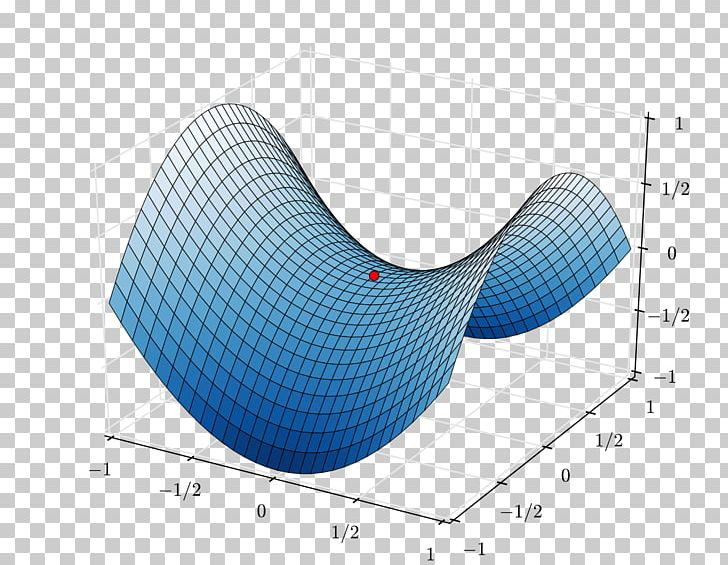
\includegraphics[height=3.7cm]{saddle-point.jpg}
  \end{center}
\end{frame}

\begin{frame}{Proof}

  \textbf{Proof [$\star$]:}
  (I) $x^\star\in \arg\min_{x\in X} ~L(x, F^\star)$. We have that $f(x^\star)\leq L(x, F^\star)$ as $F^\star$ is dual feasible. We also have $f(x^\star) = F^\star(b) = F^\star(g(x^\star))$ from the previous theorem.  Hence, $f(x^\star) = L(x^\star, F^\star)$. (II)
  $F^\star \in \arg \max_{F\in \mc F} ~L(x^\star, F)$. We have that $f(x^\star)\geq L(x^\star, F)$ for any $F\in \mc F$ as $x^\star$ is primal feasible. Again from the previous theorem, $F^\star(b) = L(x^\star, F^\star)$.


\end{frame}

\begin{frame}{Nonlinear Classification}

  \textbf{Nonlinear classification problem:}
  \begin{itemize}
  \item Transformation $\emph{\varphi}:\Re^p\to\Re^{p'}$ with $p'\gg p$.
  \item Training set $\{(\emph{\varphi}(x_i), y_i)\}_{i=1}^n$ : features $\emph{\varphi}(x_i)\in\Re^{p'}$ and class labels $y_i \in \{-1, 1\}$.

  \item \textbf{Classifier $h(x) = sign(\emph{\varphi}(x)\tpose w + w_0)$}
  \end{itemize}

  \vfill

  Duality:
  \[
    \begin{array}{rlcrl}
      \inf & \norm{w}_2^2/2 & = & \sup & \sum_{i=1}^n u_i - \frac12 u\tpose Q u \\[0.5em]
      \st & w\in\Re^{p'},~w_0\in\Re & & \st & u \in \Re^n_+ \\[0.5em] 
           & y_i(\varphi(x_i)\tpose w + w_0) \geq 1,~ \forall i & & & \sum_{i=1}^n u_i y_i = 0
    \end{array}
  \]
  with $Q_{ij} = y_i y_j K_{ij}$ and $K_{ij}= \iprod{\emph{\varphi}(x_i)}{\emph{\varphi}(x_j)}$ for $1\leq i, j\leq n$. Assume existence of $(w^\star, w_0^\star)$ and $u^\star$; the \emph{primal and dual optimal} solutions.
  
\end{frame}

\begin{frame}{From Dual Solution to Primal Classifier}

  \textbf{Saddle point condition:} We must have that (unconstrained optimality conditions for convex problems)
  \[
    \begin{array}{rl}
      w^\star \in \arg\min_w~ L(w, w_0^\star, u^\star) \iff w^\star= \sum_{j=1}^n u^\star_j y_j \varphi(x_j).
    \end{array}
  \]

  \vfill

  \emph{Classifier :} $h(x) = sign(\sum_{j=1}^n u^\star_j y_j K(x, x_j) + w^\star_0)$ with $K(x, x_j)=\iprod{\varphi(x)}{\varphi(x_j)}$. 

  \vfill

  \textbf{Complementarity condition:}
  \[
    \begin{array}{rl}
       &  u^\star_i  [y_i\sum_{j=1}^n  u^\star_j y_j K(x_i, x_j) + y_iw^\star_0-1]= 0 ~~\forall i \in [1,\dots, n]\\[0.5em]
      \iff &  u^\star_i  [\sum_{j=1}^n  u^\star_j y_j K(x_i, x_j) + w^\star_0-y_i]= 0~~\forall i \in [1,\dots, n]\\[0.5em]
      \implies & \sum_{i=1}^n u^\star_i  [\sum_{j=1}^n  u^\star_j y_j K(x_i, x_j) + w^\star_0-y_i] = 0\\[0.5em]
          \iff &      w^\star_0 = -\sum_{i=1}^n u^\star_i \sum_{j=1}^n u^\star_j y_j K(x_i, x_j)/(\sum_{i=1}^n u_i^\star).
    \end{array}
  \]
  
\end{frame}

\section{Constraint Qualifications}

\begin{frame}{Convex Duality}

  What happens if problem is \emph{convex}?
  \[
    \begin{array}{rlcrl}
      \inf & f(x)  & \geq & \sup & F(b) \\[0.5em]
      \st & x\in X   & &                       \st & F \in \mc F \\[0.5em]
           & g(x) \succeq_{\emph{K}} b &&    & F(g(x)) \leq f(x), ~~\forall x \in X.
    \end{array}
  \]

  That is, $f:E\to\Re$ is a convex function, $X$ a convex set, and $g$ is $K$-concave
  \[
    g(\lambda x + (1-\lambda)y) \succeq_{K} \lambda g(x) + (1-\lambda) g(y) \quad \forall x, y, ~\forall \lambda \in [0, 1]
  \]

  \vfill
  \textbf{Remarks:}
  \begin{itemize}
  \item Concavity coincides with $\Re_+$-concavity
  \item Linearity (Affine functions) coincides with $\{0\}$-concavity
  \item \emph{Most general} convex problem class
  \end{itemize}
  
\end{frame}

\begin{frame}{Conic Duality [$\star$]}

  We can rewrite any convex problem in \emph{standard form} (nice exercise!). Standard dual becomes
  \[
    \begin{array}{rl}
      \inf & \iprod{c}{x}\\
      \st & Ax = b \\
                & x\in K.
    \end{array}
    \quad \geq \quad
    \begin{array}{rl}
      \sup & \iprod{y}{b}\\
      \st & A\tpose y + s = c \\
           & s\in K^\star.
    \end{array}
  \]
  %Slater's condition translates to $\exists \bar x : A \bar x - b \in \relint K$.

  \vfill

 \uncover<2->{
  \textbf{Proof :}
  Let $\bar K = \{0\} \times K$ with dual cone $\bar K^\star = \Re^m\times K^\star$. Then,
  \begin{align*}
    \begin{array}{rl}
      \inf & \iprod{c}{x}\\
      \st & Ax = b \\
           & x\in K.
    \end{array}
    ~~ =& ~~ 
    \begin{array}{rl}
      \inf & \iprod{c}{x}\\
      \st & \begin{pmatrix} A x \\ x \end{pmatrix}\succeq_{\bar K} \begin{pmatrix} b \\ 0 \end{pmatrix} \\
    \end{array}\\
    \geq & ~~
    \begin{array}{rl}
      \sup & \iprod{u_1}{b} + u_0\\
      \st & \iprod{u_1}{A x} + \iprod{u_2}{x} + u_0 \leq \iprod{c}{x} \forall x \in \Re^n \\
           & u_1 \in \Re^m, ~u_2\in K^\star.
    \end{array}
             \intertext{Note that $u_0\leq 0$ (take $x=0$) and $u_0 < 0$ is suboptimal. So $u_0=0$.}
           =  & ~~ \begin{array}{rl}
      \sup & \iprod{y}{b}\\
      \st & A^\star y + s = c \\
           & s\in K^\star.
    \end{array}
  \end{align*}
  }
  
\end{frame}


\begin{frame}{Slater's Condition}

  \emph{Slater's condition} holds when there is point $\bar x \in \interior(X)$ such that $g(\bar x) - b \in \relint(K)$.

  \vfill
  
  \textbf{Theorem : } Under convexity and Slater's condition
  \[
    p^\star = \inf_{x\in X}\,\sup_{u\in K^\star}~f(x) + \iprod{u}{b-g(x)} = \sup_{u\in K^\star}\,\inf_{x\in X}~f(x) + \iprod{u}{b-g(x)} = d^\star
  \]

  \vfill

  \textbf{Remark:}
  \begin{itemize}
  \item Slater's condition is typically much easier to verify than the minimax property itself
  \item<2-> \emph{Sufficient} condition of strong duality 
  \end{itemize}
\end{frame}

\begin{frame}{SVM : Constraint Qualification}

  Primal and dual formulations:
  \[
    \begin{array}{rlcrl}
      \inf & \norm{w}_2^2/2 & = & \sup & \sum_{i=1}^n u_i - \frac12 \sum_{1\leq i, j \leq n}u_i u_j y_i y_j (x_i\tpose x_j) \\[0.5em]
      \st & w\in\Re^p,~w_0\in\Re & & \st & u \in \Re^n_+ \\[0.5em] 
           & y_i(x_i\tpose w + w_0) \geq 1,~ \forall i & & & \sum_{i=1}^n u_i y_i = 0
    \end{array}
  \]
  with $K_{ij}=y_iy_j\iprod{x_i}{x_j}$ for all $1\leq i, j\leq n$.
  

  \vfill

  \textbf{Strong Duality :} Take any feasible point $(w, w_0)$. The point $\gamma (w, w_0)$ for $\gamma>1$ is a \emph{Slater point}.
  
\end{frame}

\begin{frame}{When Slater Fails [$\star$]}

  \textbf{Primal:} ($p^\star = 2$).
  \[
    \begin{array}{rl}
      p^\star = \min & 2 x_3 - 2 x_4\\[0.5em]
      \st & x_3 + x_4 = 1, ~x_2 = 0,\\[0.5em]
           &
             \begin{pmatrix}
               x_1 & x_4 & x_6\\
               x_4 & x_2 & x_5\\
               x_6 & x_5 & x_3
             \end{pmatrix}
                           \in S^3_+.\hspace{9em}
    \end{array}
  \]

  \vfill

  \textbf{Dual:} ($d^\star=-2$)
  \[
    \begin{array}{rl}
      d^\star = \max & u_1\\[0.5em]
      \st &
                       \begin{pmatrix}
                         0 & -1-u_1/2 & 0\\
                         -1-u_1/2 & -u_2 & 0\\
                         0 & 0 & 2-u_1
                       \end{pmatrix}
                                     \in S^3_+.
    \end{array}
  \]

  \vfill

  Slater's condition can not be disregarded!
  
\end{frame}

% \begin{frame}{Convexity and Duality}

%   \[
%     \begin{array}{rlcrl}
%       \inf & f(x)  & \geq & \sup & F(b) \\[0.5em]
%       \st & x\in X   & &                       \st & F \in \mc F \\[0.5em]
%            & g(x) \succeq_{\emph{K}} b &&    & F(g(x)) \leq f(x), ~~\forall x \in X.
%     \end{array}
%   \]

%   \vfill

%   \textbf{Why convexity simplifies everything:}
%   \begin{itemize}
%     \setlength\itemsep{1em}
%   \item Strong duality with simple dual functions $\mc F_{\rm{aff}}=\set{c\mapsto\iprod{u}{c}+u_0}{u\in K^\star ,~u\in\Re}$ and Slater's condition.
%   \item The Lagrangian
%     \[
%       L(x, u) = f(x) + \iprod{u}{b-g(x)}
%     \]
%     is easier to maximize in $u$ for fixed $x$. Easier to minimize in $x$ for fixed $u$.
%   \item If $f(x^\star)=\iprod{u^\star}{b}+u_0^\star$ we have the saddle point
%     \[
%       f(x^\star) = \min_{x\in X}~ L(x, u^\star), \quad \iprod{u^\star}{b} = \max_{~u\in K^\star} ~L(x^\star, u).
%     \]
%   \end{itemize}
  
% \end{frame}

\end{document}
%%% Local Variables:
%%% mode: latex
%%% TeX-master: t
%%% End:
